% ---
% Capa
% ---
\imprimircapa
% ---

% ---
% Folha de rosto
% (o * indica que haverá a ficha bibliográfica)
% ---
\imprimirfolhaderosto*
% ---

% ---
% Inserir a ficha bibliografica
% ---
% http://ficha.bu.ufsc.br/
%\begin{fichacatalografica}
%	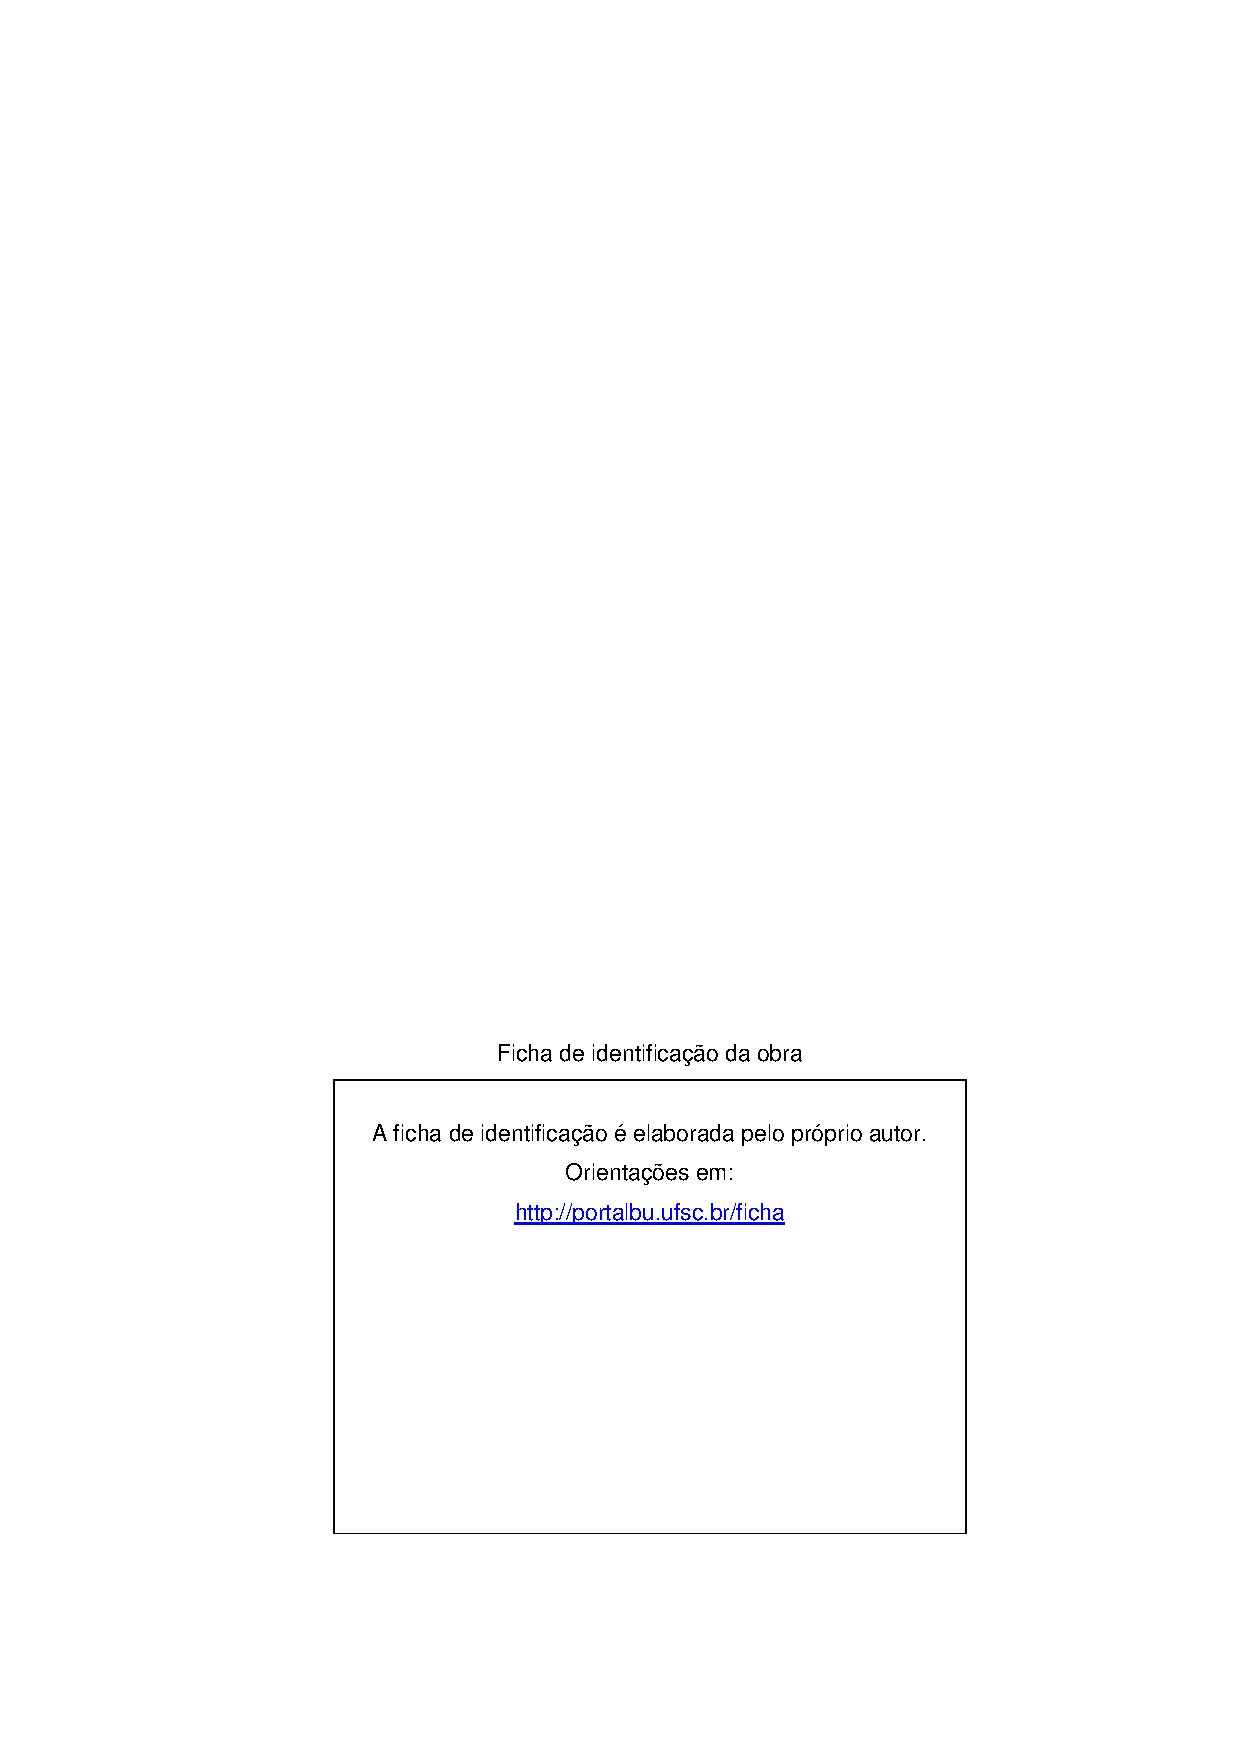
\includepdf{beforetext/Ficha_Catalografica.pdf}
%\end{fichacatalografica}
% ---

% ---
% Inserir folha de aprovação
% ---
%\begin{folhadeaprovacao}
	%\OnehalfSpacing
	%\centering
	%\imprimirautor\\%
	%\vspace*{10pt}		
	%\textbf{\imprimirtitulo}%
	%\ifnotempty{\imprimirsubtitulo}{:~\imprimirsubtitulo}\\%
	%		\vspace*{31.5pt}%3\baselineskip
	%\vspace*{\baselineskip}
	%\begin{minipage}{\textwidth}
	%% ~do~\imprimirprograma~do~\imprimircentro~da~\imprimirinstituicao~para~a~obtenção~do~título~de~\imprimirformacao.
	%Este~\imprimirtipotrabalho~foi julgado adequado para obtenção do Título de “\imprimirformacao” e aprovado em sua forma final pelo~\imprimirprograma. \\
	%	\vspace*{\baselineskip}
	%\imprimirlocal, \imprimirdata. \\
	%\vspace*{2\baselineskip}
	%\assinatura{\OnehalfSpacing\imprimircoordenador \\ %\imprimircoordenadorRotulo~do Curso}
	%\vspace*{2\baselineskip}
	%\textbf{Banca Examinadora:} \\
	%\vspace*{\baselineskip}
	%\assinatura{\OnehalfSpacing\imprimirorientador \\ %\imprimirorientadorRotulo}
%	%\end{minipage}%
%	\vspace*{\baselineskip}
%	\assinatura{Prof.(a) xxxx, Dr(a).\\
%	Avaliador(a) \\
%	Instituição xxxx}

%	\vspace*{\baselineskip}
%	\assinatura{Prof.(a) xxxx, Dr(a).\\
%	Avaliador(a) \\
%	Instituição xxxx}


%\end{folhadeaprovacao}

\begin{folhadeaprovacao}

	%\begin{snugshade}
	%\begin{center}
	%{\textbf{\small{FOLHA DE APROVAÇÃO DE PROPOSTA DE TCC}}}
	%\end{center}
	%\end{snugshade}
    %\vspace{-22pt}
    
    
    \begin{quadro}[htb]
	\centering
	\label{qua:folha_aprov_title}
	%\caption{\label{qua:folha_aprov}Formatação do texto.}	
	\begin{tabular}{ p{\textwidth}}
		\hline
		\cellcolor{shadecolor} \textbf{\small{FOLHA DE APROVAÇÃO DE PROPOSTA DE TCC}}\\ \hline
   
	\end{tabular}
	%\fonte{\textcite{NBR14724:2011}.}
\end{quadro}

\vspace{-22pt}

\begin{quadro}[htb]
	\centering
	\label{qua:folha_aprov}
	%\caption{\label{qua:folha_aprov}Formatação do texto.}	
	\begin{tabular}{|l|p{11cm}|}
		\hline
		\textbf{Acadêmico} & \imprimirautor\\ \hline
		\textbf{Título do trabalho}        & \imprimirtitulo\\ \hline
		\textbf{Curso}          & \imprimirprograma\\ \hline
		\textbf{Área de Concentração}        & Compressão de Vídeo  \\ \hline    
	\end{tabular}
	%\fonte{\textcite{NBR14724:2011}.}
\end{quadro}

\vspace{-15pt}

	\noindent \textbf{Instruções para preenchimento pelo \small{ORIENTADOR DO TRABALHO}:}
	\begin{itemize}[leftmargin=*,noitemsep,topsep=0pt]
		\item[-] \small Para cada critério avaliado, assinale um X na coluna SIM apenas se considerado aprovado. Caso contrário, indique as alterações necessárias na coluna Observação.
	\end{itemize}

\vspace{5pt}

	\noindent\resizebox{\textwidth}{!}{
		\centering
		\begin{tabular}{|X p{6.5cm}|X p{0.7cm}|X p{1.5cm}|X p{0.7cm}|X p{1.5cm}|X p{5.2cm}|}
			%\begin{small}\hhline{*{1}{{|~}*{4}{\arrayrulecolor{shadecolor}|-}|~}
				\hline
				%\multirow{2}{*}{\textbf{Critérios}} &  \textbf{Sim} &  \textbf{Parcial} &  \textbf{Não} &  \textbf{Não se aplica} & \multirow{2}{*}{\textbf{Observação}}\\ \hline{>{\arrayrulecolor{shadecolor}}}
			    \cellcolor{shadecolor} & \multicolumn{4}{c|}{\cellcolor{shadecolor} \textbf{Aprovado}} & \cellcolor{shadecolor} \\ \hhline{*{1}{>{\arrayrulecolor{shadecolor}}-}*{4}{>{\arrayrulecolor{black}}|-}>{\arrayrulecolor{shadecolor}}|->{\arrayrulecolor{black}}}
			    \multirow{-1}{*}{\cellcolor{shadecolor} {\small \textbf{Critérios}}} & \cellcolor{shadecolor} {\small \textbf{Sim}} &  \cellcolor{shadecolor} {\small \textbf{Parcial}} &  \cellcolor{shadecolor} {\small \textbf{Não}} &  \cellcolor{shadecolor} {\small \textbf{Não se aplica}} & \multirow{-1}{*}{\cellcolor{shadecolor} {\small \textbf{Observação}}} \\ \hline
				{\small 1.O trabalho é adequado para um TCC no CCO/SIN (relevância/abrangência)?} & \cellcolor{shadecolor} X & \cellcolor{shadecolor}  & \cellcolor{shadecolor}  & \cellcolor{shadecolor}  & \\ \hline
				{\small 2.O título do trabalho é adequado?} & \cellcolor{shadecolor} X & \cellcolor{shadecolor}  & \cellcolor{shadecolor}  & \cellcolor{shadecolor}  & \\ \hline
				{\small 3.O tema de pesquisa está claramente descrito?} & \cellcolor{shadecolor} X & \cellcolor{shadecolor}  & \cellcolor{shadecolor}  & \cellcolor{shadecolor}  & \\ \hline
				{\small 4.O problema/hipóteses de pesquisa do trabalho está claramente identificado?} & \cellcolor{shadecolor} X & \cellcolor{shadecolor}  & \cellcolor{shadecolor}  & \cellcolor{shadecolor}  & \\ \hline
				{\small 5.A relevância da pesquisa é justificada?} & \cellcolor{shadecolor} X & \cellcolor{shadecolor}  & \cellcolor{shadecolor}  & \cellcolor{shadecolor}  & \\ \hline
				{\small 6.Os objetivos descrevem completa e claramente o que se pretende alcançar neste trabalho?} & \cellcolor{shadecolor} X & \cellcolor{shadecolor}  & \cellcolor{shadecolor}  & \cellcolor{shadecolor}  & \\ \hline
				{\small 7.É definido o método a ser adotado no trabalho? O método condiz com os objetivos e é adequado para um TCC? } & \cellcolor{shadecolor} X & \cellcolor{shadecolor}  & \cellcolor{shadecolor}  & \cellcolor{shadecolor}  & \\ \hline
				{\small 8.Foi definido um cronograma coerente com o método definido (indicando todas as atividades) e com as datas das entregas (p.ex.Projeto I, II, Defesa)?} & \cellcolor{shadecolor} X & \cellcolor{shadecolor}  & \cellcolor{shadecolor}  & \cellcolor{shadecolor}  & \\ \hline
				{\small 9.Foram identificados custos relativos à execução deste trabalho (se houver)? Haverá financiamento para estes custos?} & \cellcolor{shadecolor} X & \cellcolor{shadecolor}  & \cellcolor{shadecolor}  & \cellcolor{shadecolor}  & \\ \hline
				{\small 10.Foram identificados todos os envolvidos neste trabalho?} & \cellcolor{shadecolor} X & \cellcolor{shadecolor}  & \cellcolor{shadecolor}  & \cellcolor{shadecolor}  & \\ \hline
				{\small 11.As formas de comunicação foram definidas (ex: horários para orientação)?} & \cellcolor{shadecolor} X & \cellcolor{shadecolor}  & \cellcolor{shadecolor}  & \cellcolor{shadecolor}  & \\ \hline
				{\small 12.Riscos potenciais que podem causar desvios do plano foram identificados?} & \cellcolor{shadecolor} X & \cellcolor{shadecolor}  & \cellcolor{shadecolor}  & \cellcolor{shadecolor}  & \\ \hline
				{\small 13.Caso o TCC envolva a produção de um software ou outro tipo de produto e seja desenvolvido também como uma atividade	realizada numa empresa ou laboratório, consta da proposta uma declaração (Anexo A) de ciência e concordância com a entrega do código fonte e/ou documentação produzidos? } & \cellcolor{shadecolor} X & \cellcolor{shadecolor}  & \cellcolor{shadecolor}  & \cellcolor{shadecolor}  & \\ \hline

			%\end{small}
		\end{tabular}
	}

\vspace{5pt}

	\noindent\resizebox{\textwidth}{!}{
		\begin{tabular}{| p{3.4cm}| p{2.35cm}| p{1.4cm}| p{5.4cm}|}
				\hline
			    {\tiny \textbf{Avaliação}} &  \multicolumn{1}{l}{\textbf{$\boxtimes$ \tiny Aprovado}}  & \multicolumn{2}{c|}{\textbf{$\Box$ \tiny Não Aprovado}}  \\ \hline \hline

			    {\tiny \textbf{Professor Responsável}} &  {\tiny Prof. Dr. José Luís A. Güntzel} & {\tiny 13/11/2023} & \\ \hline
                {\tiny \textbf{Orientador}} &  {\tiny Me. André Beims Bräscher} & {\tiny 13/11/2023} & \\ \hline

		\end{tabular}
	}


\end{folhadeaprovacao}

% ---

% ---
% Dedicatória
% ---
%\begin{dedicatoria}
%	\vspace*{\fill}
%	\noindent
%	\begin{adjustwidth*}{}{5.5cm}     
%		Este trabalho é dedicado aos meus colegas de classe e aos meus queridos pais.
%	\end{adjustwidth*}
%\end{dedicatoria}
% ---

% ---
% Agradecimentos
% ---
%\begin{agradecimentos}
%	Inserir os agradecimentos aos colaboradores à execução do trabalho. 
	
%	Xxxxxxxxxxxxxxxxxxxxxxxxxxxxxxxxxxxxxxxxxxxxxxxxxxxxxxxxxxxxxxxx. 
%\end{agradecimentos}
% ---

% ---
% Epígrafe
% ---
%\begin{epigrafe}
%	\vspace*{\fill}
%	\begin{flushright}
%		\textit{``Texto da Epígrafe.\\
%			Citação relativa ao tema do trabalho.\\
%			É opcional. A epígrafe pode também aparecer\\
%			na abertura de cada seção ou capítulo.\\
%			Deve ser elaborada de acordo com a NBR 10520.''\\
%			(Autor da epígrafe, ano)}
%	\end{flushright}
%\end{epigrafe}
% ---

% ---
% RESUMOS
% ---

% resumo em português
\setlength{\absparsep}{18pt} % ajusta o espaçamento dos parágrafos do resumo
\begin{resumo}
	\SingleSpacing
	
	%No resumo são ressaltados o objetivo da pesquisa, o método utilizado, as discussões e os resultados com destaque apenas para os pontos principais. O resumo deve ser significativo, composto de uma sequência de frases concisas, afirmativas, e não de uma enumeração de tópicos. Não deve conter citações. Deve usar o verbo na voz ativa e na terceira pessoa do singular. O texto do resumo deve ser digitado, em um único bloco, sem espaço de parágrafo. O espaçamento entre linhas é simples e o tamanho da fonte é 12. Abaixo do resumo, informar as palavras-chave (palavras ou expressões significativas retiradas do texto) ou, termos retirados de thesaurus da área. Deve conter de 150 a 500 palavras. O resumo é elaborado de acordo com a NBR 6028.

    Considerando o aumento significativo observado no consumo e compartilhamento de vídeos nos últimos anos, é notória a demanda por técnicas que permitam armazenamento, transmissão e reprodução desse tipo de dado de forma cada vez mais otimizada.
    Para essa finalidade, a abordagem mais consolidada é a codificação de vídeo híbrida, que tem sido parte essencial da área de codificação de vídeo nas últimas décadas.
    Contudo, estima-se que a complexidade de algoritmos tradicionais híbridos venha aumentando em 10X para um ganho de desempenho de 2X, a cada geração. 
    Nesse contexto, surge a necessidade de buscar modelos alternativos de codificação, como o \ac{DIVC}. 
    O \ac{DIVC} combina o modelo de codificação híbrido com \ac{VFI}, porém tem desempenho variável de acordo com o conteúdo do vídeo.
    Portanto, o objetivo deste trabalho é propor uma técnica para melhorar sua eficiência de codificação a partir da remoção de quadros de forma adaptativa. Para isso, os quadros serão analisados utilizando descritores que apresentem melhor correlação com a eficiência do modelo.
    
    \textbf{Palavras-chave:} Codificação de vídeo. VVC. Eficiência de codificação. Descritores de imagem. VFI. Redes Neurais.
\end{resumo}

% resumo em inglês
%\begin{resumo}[Abstract]
%	\SingleSpacing
%	\begin{otherlanguage*}{english}
%		Resumo traduzido para outros idiomas, neste caso, inglês. Segue o formato do resumo feito na língua vernácula. As palavras-chave traduzidas, versão em língua estrangeira, são colocadas abaixo do texto precedidas pela expressão “Keywords”, separadas por ponto.
		
%		\textbf{Keywords}: Keyword 1. Keyword 2. Keyword 3.
%	\end{otherlanguage*}
%\end{resumo}

%% resumo em francês 
%\begin{resumo}[Résumé]
% \begin{otherlanguage*}{french}
%    Il s'agit d'un résumé en français.
% 
%   \textbf{Mots-clés}: latex. abntex. publication de textes.
% \end{otherlanguage*}
%\end{resumo}
%
%% resumo em espanhol
%\begin{resumo}[Resumen]
% \begin{otherlanguage*}{spanish}
%   Este es el resumen en español.
%  
%   \textbf{Palabras clave}: latex. abntex. publicación de textos.
% \end{otherlanguage*}
%\end{resumo}
%% ---

{%hidelinks
	\hypersetup{hidelinks}
	% ---
	% inserir lista de ilustrações
	% ---
	\pdfbookmark[0]{\listfigurename}{lof}
	% \listoffigures*
	\cleardoublepage
	% ---
	
	% ---
	% inserir lista de quadros
	% ---
	%\pdfbookmark[0]{\listofquadrosname}{loq}
	%\listofquadros*
	%\cleardoublepage
	% ---
	
	% ---
	% inserir lista de tabelas
	% ---
	%\pdfbookmark[0]{\listtablename}{lot}
	%\listoftables*
	%\cleardoublepage
	% ---
	
	% ---
	% inserir lista de abreviaturas e siglas (devem ser declarados no preambulo)
	% ---
	\imprimirlistadesiglas
	% ---
	
	% ---
	% inserir lista de símbolos (devem ser declarados no preambulo)
	% ---
	%\imprimirlistadesimbolos
	% ---
	
	% ---
	% inserir o sumario
	% ---
	\pdfbookmark[0]{\contentsname}{toc}
	\tableofcontents*
	\cleardoublepage
	
}%hidelinks
% ---